\section{Results}
EMD on the 3 signals introduced in Section \ref{problem}
Using EMD we show that the 3 signals have a common weekly pattern, however, only two signals are correlated at smaller time scales.

\subsection{Data de-trending}
\begin{table*}
\begin{center}
\begin{tabular}{|l|l|l|l|l|l|}
\hline
× & Original data & 1st IMF & 2nd IMF & 3rd IMF & Residual\\ \hline
EHP, Light & 0.7720 & 0.4431 & 0.5104 & 0.6171 & 0.8114\\ \hline
EHP, GHP & 0.6369 & -0.0055 & 0.0883 & 0.2350 & 0.7956\\ \hline
\end{tabular}

\caption{Correlation coefficients of the analyzed signal and their IMF uncovered by EMD}

\end{center}
\end{table*}

Speak about the three IMFs and their correlation coefficients.



\subsection{}
\begin{figure*}
\centering
 \subfigure[Raw signals correlation coefficients]{\includegraphics[width=.45\textwidth]{img/allFloors_week1_week4_corr_abs.eps}}
 \subfigure[Average IMFs correlation coefficients]{\includegraphics[width=.45\textwidth]{img/allFloors_week1_week4_emd_abs.eps}}
 \caption{Distribution of the correlation coefficients of the raw signals and corresponding IMFs using 3 weeks of data from 674 sensors deployed on 12 Floors.}
\end{figure*}
